\documentclass[10pt]{article}
\setlength{\parskip}{0.25\baselineskip}
\usepackage[margin=1in]{geometry} 
\usepackage{amsmath,amsthm,amssymb, graphicx, multicol, array}
\usepackage[font=small,labelfont=bf]{caption}
\usepackage{float}

\newcommand{\supp}{{\text{supp}}} 
\newcommand{\bv}{{\text{BV}}}
\newcommand{\ac}{{\text{AC}}}

\newenvironment{problem}[2][]{\begin{trivlist}
\item[\hskip \labelsep {\bfseries #1}\hskip \labelsep {\bfseries #2.}]}{\end{trivlist}}

\begin{document}
 
\title{Homework \#4}
\author{Eric Tao\\
Math 123: Homework \#4}
\maketitle

\begin{problem}{Question 1}

Let $\{ x_i \}_{i=1}^n \subset \mathbb{R}^D$. Define $F: \mathbb{R}^D \to [0,\infty)$ via:

$$ F(y) = \sum_{i=1}^n \Vert x_i - y \Vert_2^2$$

Prove that $F$ attains a minimum at $y = \frac{1}{n} \sum_{i=1}^n x_i$.
\end{problem}
\begin{proof}[Solution]

First, we rewrite:

$$F(y) = \sum_{i=1}^n \sum_{j=1}^D (x_{i_j} - y_j)^2$$

Well, here, we take the derivative $\frac{dF}{dy}$, and in particular, we look at the $y_i$-th term. 

$$ \frac{dF}{dy_k} =  \sum_{i=1}^n \frac{\partial}{\partial y_k} \sum_{j=1}^D  (x_{i_j} - y_j)^2 = \sum_{i=1}^n -2(x_{i_k} -  y_k) $$

Setting this equal to 0, we have that:

$$  \sum_{i=1}^n -2(x_{i_k} - y_k)  = 0 \implies \sum_{i=1}^n (x_{i_k} - y_k)  = 0  \implies - n y_k + \sum_{i=1}^n x_{i_k} = 0 \implies y_k = \frac{1}{n}  \sum_{i=1}^n x_{i_k} $$

Since this is true across $y_k$, we have then that $y = \frac{1}{n} \sum_{i=1}^n x_i$ as vectors, as desired.

\end{proof}

\begin{problem}{Question 2}

Suppose $x_1,...,x_n \in \mathbb{R}^D$ are data points, and we introduce an outlier $x^o$ with the property that, for some $\delta > 0$, $\Vert x_i  - x^o \Vert_2 > \delta$ for all $i$. Suppose we run K-means on this data set with $K = 2$.

(a) Argue that as $\delta \to + \infty$, that one of the clusters learned by K-means will consist of the singleton $\{ x^o \}$.

(b) This lack of robustness to outliers is sometimes considered a defect of K-means. Suggest some changes to the K-means algorithm to improve its robustness to outliers.

(c) Instead of thinking of the lack of robustness to outliers as a defect, can you think of any reasons it may be a virtue?

\end{problem}

\begin{proof}[Solution]

(a)

First, suppose that the maximum distance between $x_i$ and $\mu$, for $\mu$ the mean of $\{ x_i \}_{i=1}^n$ is $M$, which we can do since we have a finite set of data points, and thus a finite set of distances.

Suppose we have a point $x^o$ such that $\Vert x_i  - x^o \Vert_2 > \delta$, for all other points $x_i$. Then, consider the value of the functional when $x^o$ is in a cluster by itself, and arbitrarily assume this is $C_2$, by labeling. We would have that:

$$ F(C_1,C_2) = \sum_{x_i \in C_1} \Vert x_i - \mu_1 \Vert_2^2 + \Vert x^o - x^o \Vert_2^2 \leq  \sum_{x_i \in C_1} M^2 = nM^2$$

First, suppose $n=1$. Then, of course the only permissable partition is $C_1 = \{ x_1 \}, C_2 = \{ x^o \}$ as any other attempt would have an empty set.

Now, suppose $n \geq 2$.

Now, suppose $x^o$ were not in a singleton cluster. Suppose we had $m < n$ points in $C_1$. Then, we would have that:

$$  F'(C_1,C_2) = \sum_{x_i \in C_1} \Vert x_i - \mu'_1 \Vert_2^2 + \sum_{x_i \in C_2} \Vert x_i - \mu'_2 \Vert_2^2 + \Vert x^o - \mu'_2 \Vert_2^2$$

Now, since the choice of $\delta$ can be made arbitrarily large, choose $\delta$ such that $\delta > 2nM > 0$.

Then, we have that:

$$ \Vert x^o - \mu'_2 \Vert_2^2 \geq \frac{2nM}{2}^2 = n^2M^2 > nM^2$$

since any centroid for $C_2$ must be at least halfway between $x^o$ and any $x_j \in C_2$.

But, we have that  $F'$ is a sum of non-negative numbers, so we have that:

$$ F' \geq n^2 M^2 > nM^2 \geq F$$

Thus, if we assume k-means converges, with a suitable number of replicants, then for $\delta$ large enough, $x^o$ should be in its own cluster.

(b)

If we had concerns about outliers, the natural course of action would be to cluster using an approach via medians or scrub the data of outliers, i.e. remove data points where $\delta > 2nM$. A median may involve instead of using the mean, taking the median of the coordinates in order to reduce the effect of the outlier on the centroid. These are some ideas, but it is not clear a priori that these actions will preserve the structure desired from the dataset.

(c)

On the other hand, this could be considered a virtue in terms of $k$-means clustering. If we may identify outliers as their own clusters, it may imply that we should have more than $2$ clusters in our data sets, and have outlier clusters considered as well. It also may imply that the data set is not rich enough to identify true structures from the underlying source.


\end{proof}

\begin{problem}{Question 3}

K-means is often combined with a feature extraction step in which the data to be clustered is first transformed to a more convenient form. As the course progresses, we will consider some data-dependent feature extraction methods, but for now, let us consider a very particular feature extraction method: converting Cartesian to polar coordinates in $\mathbb{R}^2$.

(a) Load the data in 'CircularK\_Means.m', and run K-means with $K=2$, displaying your labels as colors on the plotted data. In terms of the K-means functional, why does this method produce the "incorrect" clusters it does?

(b) Convert the data to polar coordinates and re-run K-means to show that the data may be labeled properly in this way.

(c) Explain what about the polar coordinate representation is convenient for this data.

\end{problem}

\begin{proof}[Solution]

Running $K$-means on the circular data, we get something like this:

\begin{figure}[H]
\centering
\begin{minipage}{.5\textwidth}
  \centering
  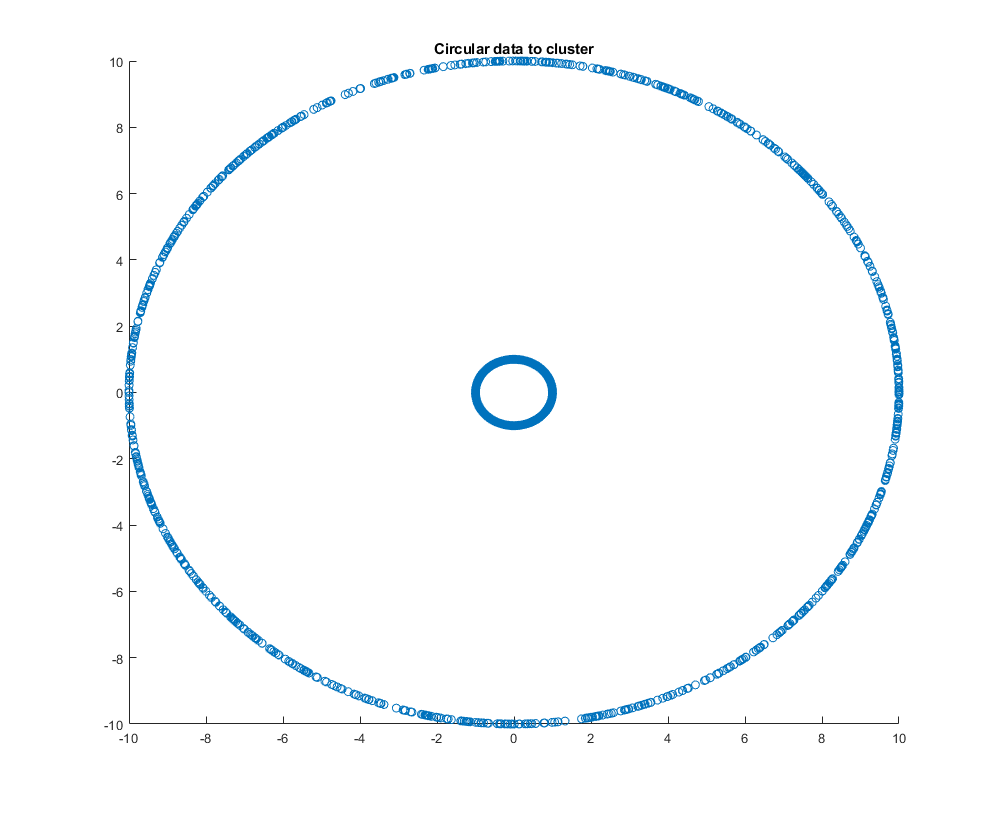
\includegraphics[width=\linewidth]{k_means_circular_raw_points}
  \captionof{figure}{Circular points}
  \label{fig:test1}
\end{minipage}%
\begin{minipage}{.5\textwidth}
  \centering
  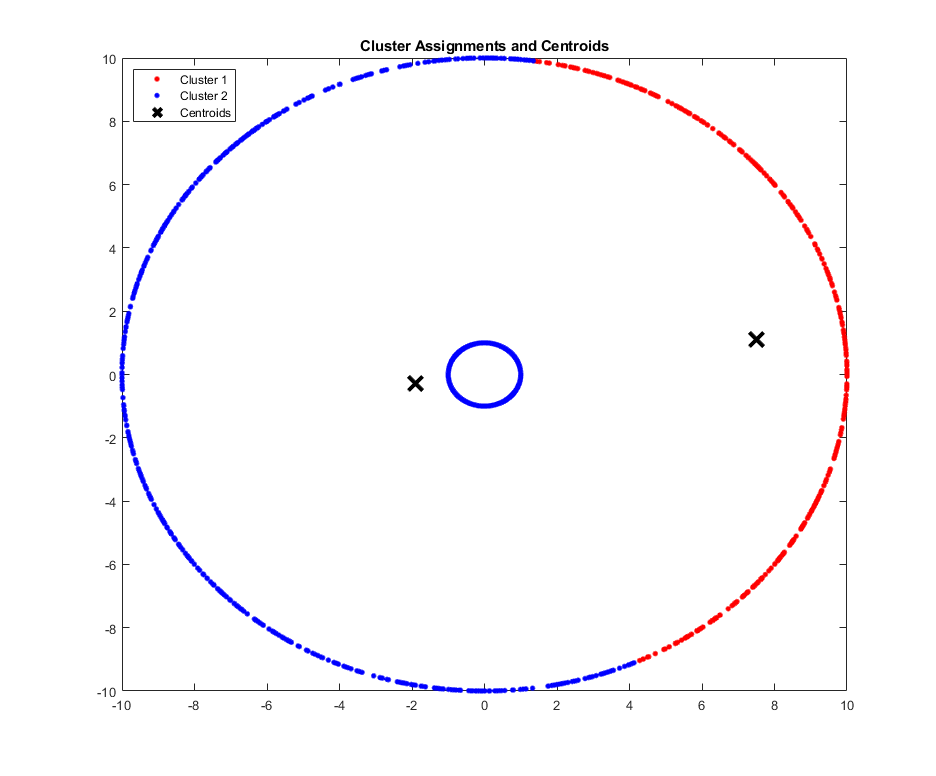
\includegraphics[width=\linewidth]{k_means_circular_with_assignment}
  \captionof{figure}{Circular points with Centroids and Cluster assignments}
  \label{fig:test2}
\end{minipage}
\end{figure}

In terms of the $K$ means functional, we get this kind of clustering because in rectangular coordinates, the geometric picture of this is of concentric circles. However, the functional is looking for essentially open balls centered at $\mu_1, \mu_2$ due to minimizing with respect to the Euclidean distance, which doesn't really work with nested data. Thus, the algorithm finds these partitions of the data because of how, geometrically, these centers minimize the open balls centered at those points, even though our data points have structure that is not captured in rectangular coordinates.

On the other hand, if we convert to polar coordinates, we find the following:

\begin{figure}[H]
\centering
\begin{minipage}{.5\textwidth}
  \centering
  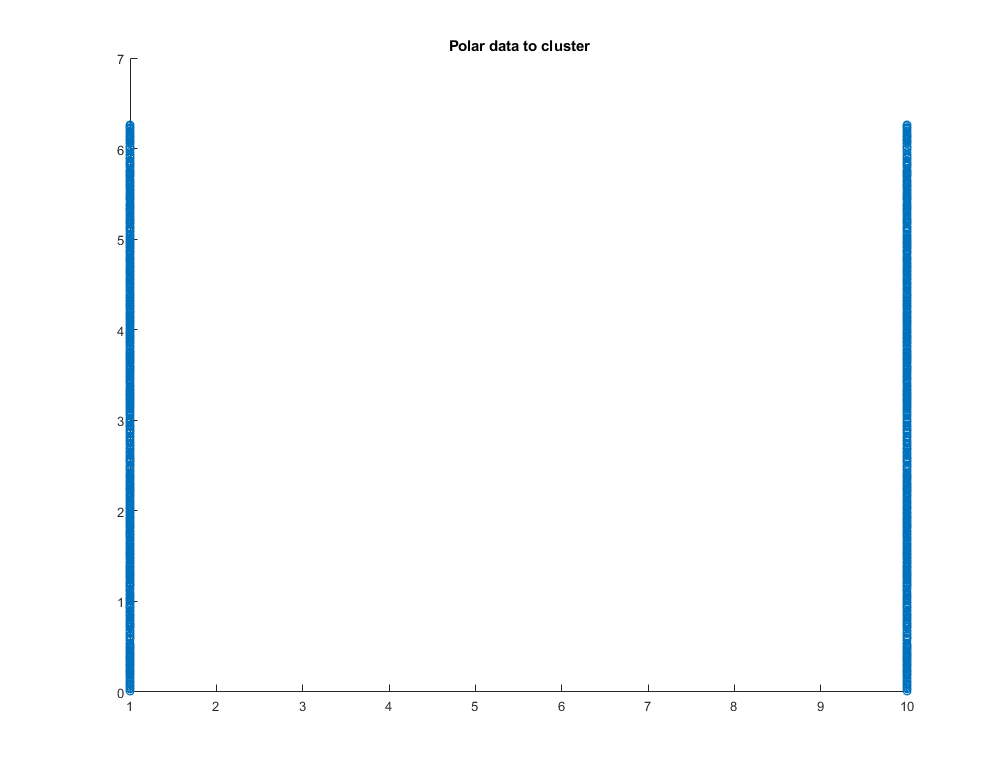
\includegraphics[width=\linewidth]{polar_circular_data}
  \captionof{figure}{Circular points in polar coordinates}
  \label{fig:test1}
\end{minipage}%
\begin{minipage}{.5\textwidth}
  \centering
  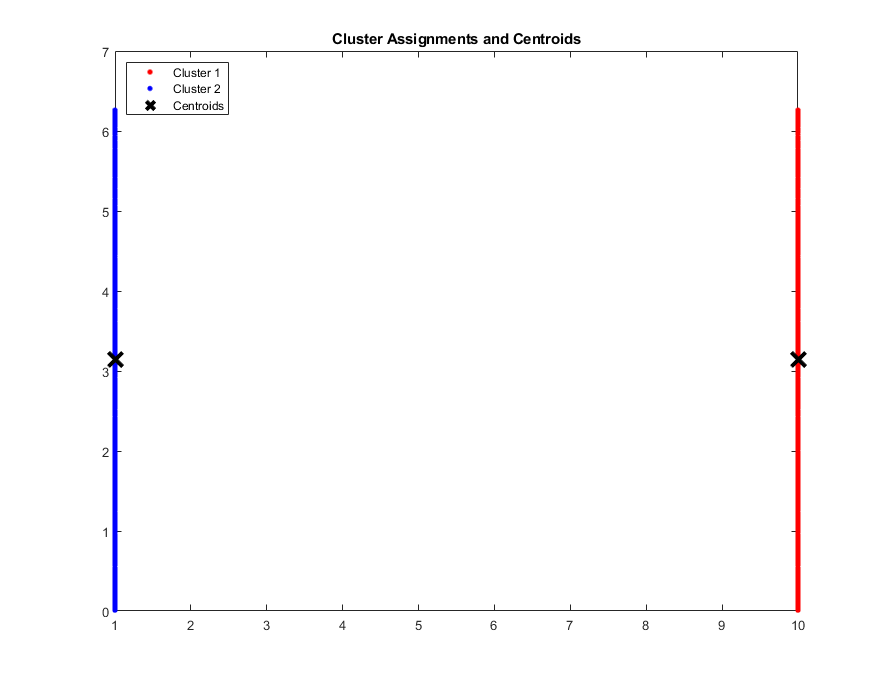
\includegraphics[width=\linewidth]{polar_cluster_assignments}
  \captionof{figure}{Circular points with Centroids and Cluster assignments in polar coordinates}
  \label{fig:test2}
\end{minipage}
\end{figure}

Here, we see that the labels are what we expect. This representation is convenient for this data because we don't have any sort of nesting structure any more, so the algorithm doesn't have issues with centering balls on the centroid to capture variance.

\end{proof}

\begin{problem}{Question 4}

(a) In MATLAB, create a data in which single linkage and complete linkage hierarchical clustering differ substantionally. Demonstrate this by conmputing the dendrograms using the built-in 'linkage' function in MATLAB, and argue that they capture different structure in the data.

(b) Argue why the two linkage methods differ on this data set in terms of their mathematical definitions.

\end{problem}

\begin{proof}[Solution]

Here, we use the same dataset as in question 3, that is, circular data, with one modification. We have the first data set at a radius of $1$, and the second to be a radius of $2$, so that the distance between the data sets is comparable to the radius of each circle. The results are as follows. noting that the clusters in the right-hand figures are the last clusters to be merged:

\begin{figure}[H]
\centering
\begin{minipage}{.5\textwidth}
  \centering
  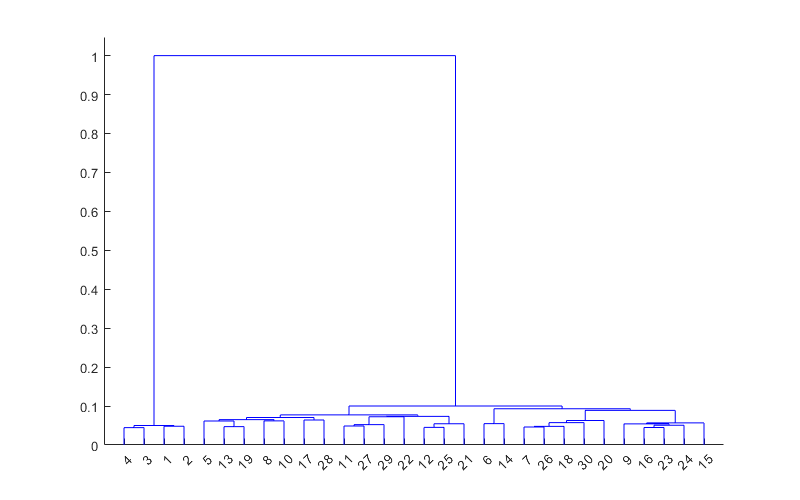
\includegraphics[width=\linewidth]{single_linkage_dendro}
  \captionof{figure}{Single Linkage Dendrogram of Circular data}
  \label{fig:test1}
\end{minipage}%
\begin{minipage}{.5\textwidth}
  \centering
  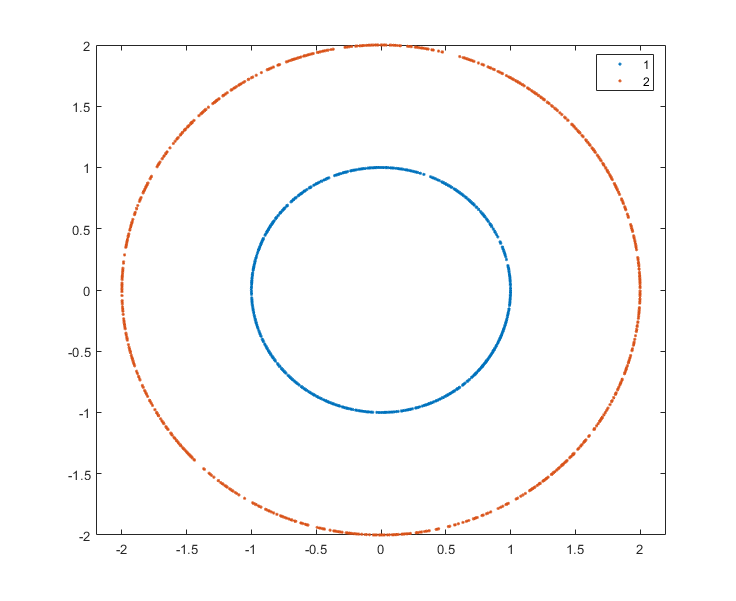
\includegraphics[width=\linewidth]{single_linkage_clusters}
  \captionof{figure}{Single Linkage Clusters of Circular data}
  \label{fig:test2}
\end{minipage}
\end{figure}

\begin{figure}[H]
\centering
\begin{minipage}{.5\textwidth}
  \centering
  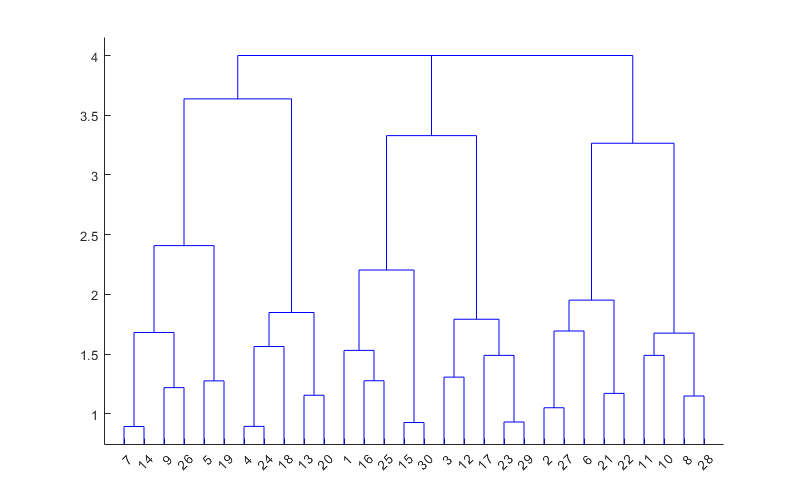
\includegraphics[width=\linewidth]{complete_linkage_dendro}
  \captionof{figure}{Complete Linkage Dendrogram of Circular data}
  \label{fig:test1}
\end{minipage}%
\begin{minipage}{.5\textwidth}
  \centering
  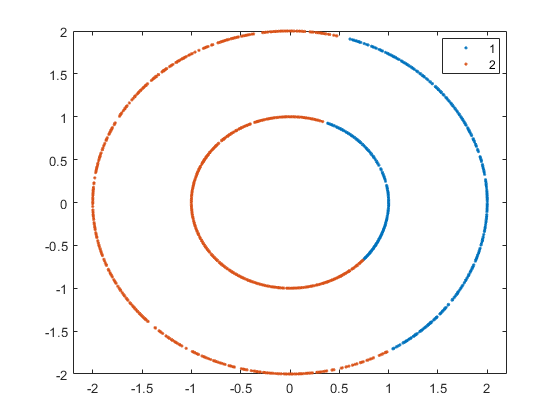
\includegraphics[width=\linewidth]{complete_linkage_clusters}
  \captionof{figure}{Complete Linkage Clusters of Circular data}
  \label{fig:test2}
\end{minipage}
\end{figure}

Here, we can see that we're capturing slightly different structure in the data. The single linkage is closer to the clustering that a polar coordinate $K$-means would capture, that is, data that is close when it is close to its nearest neighbor.

In contrast, complete linkage resembles the $K$-means when run on rectangular coordinates. In this sense, it creates the most compact clusters it could, such that no point is "far," in a sense, from each other.

Intuitively, we think about it as in complete linkage, at some point, the distance between the inner and outer rings is less than the smallest chord on a specific ring, and then complete linkage will include a point on each ring. Whereas, in single linkage, the minimum distance between points on the same ring is always less than the distance separating the rings.

\end{proof}


\end{document}